\documentclass[tikz,border=10pt]{standalone}

\begin{document}

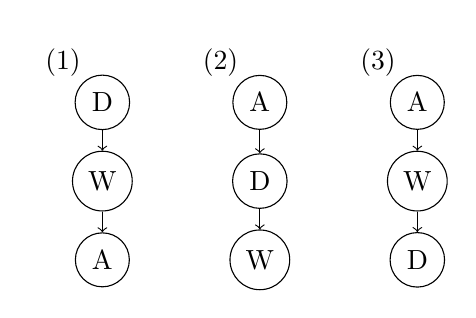
\begin{tikzpicture}[node distance=1.5cm, every node/.style={draw, circle},scale=1]

    % Chain 1
    \node (D1) at (0, 2) {D};
    \node (W1) at (0, 1) {W};
    \node (A1) at (0, 0) {A};
    \draw[->] (D1) -- (W1);
    \draw[->] (W1) -- (A1);
    \node[draw=none] at (-0.5, 2.5) {(1)};
    
    % Chain 2
    \node (A2) at (2, 2) {A};
    \node (D2) at (2, 1) {D};
    \node (W2) at (2, 0) {W};
    \draw[->] (A2) -- (D2);
    \draw[->] (D2) -- (W2);
    \node[draw=none] at (1.5, 2.5) {(2)};
    
    % Chain 3
    \node (A3) at (4, 2) {A};
    \node (W3) at (4, 1) {W};
    \node (D3) at (4, 0) {D};
    \draw[->] (A3) -- (W3);
    \draw[->] (W3) -- (D3);
    \node[draw=none] at (3.5, 2.5) {(3)};

\end{tikzpicture}

\end{document}
